%%%%%%% CICLO DI VITA COMPONENTI
\section{Ciclo di vita dei componenti}
I componenti Angular seguono il seguente lifecicle:

\begin{itemize}
    \item Istanziazione del componente e renderizzazione dello stesso e dei componenti figli all'interno del DOM
    \item Aggiornamento del componente secondo la strategia di aggiornamento al cambio delle proprietà dello stesso
    \item Distruzione del componente e dei rispettivi componenti e conseguente rimozione del componente dal DOM
\end{itemize}

È possibile definire comportamento aggiuntivo del componente ad ognuna delle fasi del ciclo di vita implementando i rispettivi metodi definiti dalla direttiva Component.
I metodi sono i seguenti:

\begin{itemize}
    \item ngOnInit() si occupa del rendering nel DOM del componente, chiamato una volta sola alla renderizzazione  del componente
    \item ngOnChanges() si occupa di aggiornare il componente quando la libreria modifica almeno una delle proprietà del componente
    \item ngOnDestroy() chiamato subito prima della distruzione di un componente
    \item ngDoCheck() per dare la possibilità di rilevare modifiche alle proprietà dei componenti che la libreria non rileva viene reso disponibile il metodo ngDoCheck() che permette di implementare la strategia di rendering desiderata 
\end{itemize}

Le chiamate ai metodi ngOnChanges() e ngDoCheck() se definiti avvengono molto di frequente nella vita di un componente portando a importanti cali di prestazioni in caso di implementazioni esose dei metodi. In particolare, il metodo ngDoCheck() viene chiamato con estrema frequenza a ogni ciclo di scansione del DOM, anche se il componente non ha subito cambiamenti.
\begin{figure}[H]
    \centering
 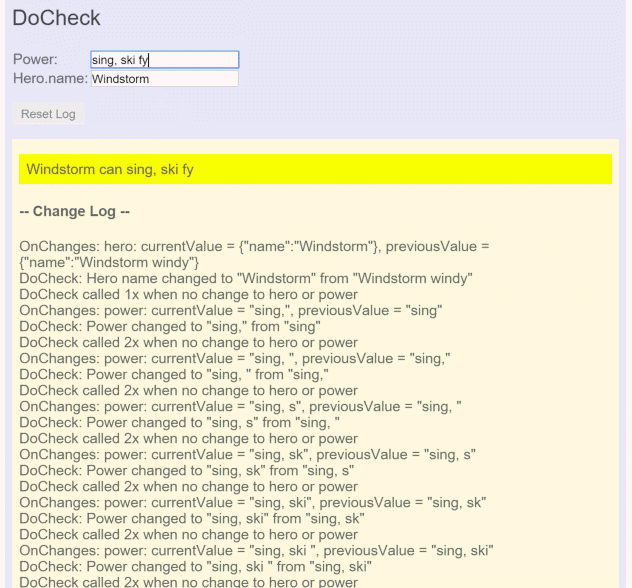
\includegraphics[scale=0.5]{resources/doCheck.png}
 \cite{angular-doc}
    \caption{funzionamento metodo ngDocheck()}
\end{figure}
come si può vedere nell'esempio, il metodo  ngDoCHeck viene chiamato diverse decine di volte anche se non avviene nessuna variazione ai valori dei due campi input.
\newline
Il metodo ngOnInit() è fondamentale nel caso di fetch di dati da un servizio remoto, essendo chiamato alla visualizzazione del componente consente di ritardare il fetch dei dati al momento in cui ce n'è un vero bisogno ed evitare il costoso fetch dei dati da parte del costruttore che rallenterebbe di molto i tempi di load dell'applicazione.
\newline
\newline
Il metodo NgOnDestroy() risulta utile per evitare memory leaks rimuovendo il componente da eventuali emettitori di eventi.
